\documentclass[twocolumn]{article}
\usepackage{amsmath}
\usepackage{algorithmic}
\usepackage{graphicx}
\date{}

\begin{document}

\title{ Implementing distributed real-time version control \\in regular expressions }

\author{Victor Grishchenko \\ \small Delft University of Technology, Ural State University }

\maketitle

\begin{abstract}
While text versioning was definitely a part of the original
hypertext concept, it is rarely considered in this context today.
Still, we know that revision control underlies the most exciting
social co-authoring projects of today's Internet, namely the
Wikipedia and the Linux kernel. With an intention to adapt the
advanced revision control technologies and practices to the
conditions of the Open Web, the paper reconsiders some obsolete
assumptions and develops a versioned text format which allows to
implement even advanced revision control operations in standard
regular expressions (pcre).

The resulting \emph{deep} hypertext model extends the linking
concept from inter-document associations to intra-document
dependencies and evolution. As the most promising consequence,
it allows decentralized real-time revision control in the Open
Web, i.e. co-evolution and mutation exchange among multiple
competing copies of the same text. 

During the last decade, on par with the process of linking diverse documents to form a single hypertext Web we have witnessed a new and promising process of synthesizing multiple points of view into a single readable text. While Google focuses on ranking, Wikipedia does merging.

That social knowledge fusion process definitely resolves some Web scalability problems simply by putting information into a easily consumable form. Still, with the current imperfect tools the new approach hit a scalability wall~\cite{wp-scale}.

To resolve the problem we look into the technological foundation of the approach, namely revision control technologies. It turns out, Wikipedia's version control is lagging 20 years behind the state of the art in the source code management (SCM) field. 

The focal point of the paper is adaptation of advanced version control technologies for Open-Web hypertext versioning. As a result, we come up with a vision of \emph{deeper} hypertext carrying its history and authorship attributions... each document representing a web itself.
The concept is proven by architected relying on regular expressions to be practical even in the constrained environment of a Web browser.


The introduction of online hypertext caused an explosion of interlinked online documents. While the Web may scale indefinitely, its practical usability faces a scalability limitation of a different sort: a user cannot consume that amount of documents, be they relevant or not, thus resorting to Google to pick the most relevant one. During the last decade we've also seen a new promising approach demonstrated by Wikipedia. It manages to synthesize readable documents by merging masses of small contributions made by different users, thus overcoming the can't-eat-it limitation. Still, Wikipedia faces scalability challenges of its own: the merge process is inherently social and complex and Wikipedia's technology apparently hit its limits of scalability as well\cite{wp-scale}.

To empower the social knowledge fusion process we turn to the well-studied area of Source Code Management for better collaboration technologies.
Generalize hypertext to build a web of contributions finally resulting in a single readable text.
The historical Xanadu vision involved some sort of versioning and attribution.

borrow from the well-studied area of SCM.
adapt revision control technologies for the conditions of the Open Web.
Thereby the paper presents a novel version control technology implemented in regular expressions and thus having native performance even in the restricted sandbox of a Web browser's JavaScript engine.
Even more importantly, the technology relies on data format... exchange versioned content on the Open Web, ... textile.
Deeper understanding of hypertext as interconnected net of contributions.!!!

Technically, the process of synthesis relies on such ... previously well-studied in the domain of source code management (SCM).
applicability of those technologies to the hypertext authoring domain and what is more important making them applicable in the Open Web in distributed fashion.
Causal trees in regular expressions... distributed version control... implemented within a browser.


social process  another aspect synthesis  
textual structure  change management attribution   alternate versions
 version control domain   source code management
technology and formats suitable for the Open Web

Two recent trends in version control systems are real-time version control and distributed version control. While the former facilitates real-time collaboration, the latter, quite to the contrary, facilitates coordination of parallel semi-independent development efforts. These changes lead to reconsideration of certain historical approaches and classical problems of version control.
Namely, the classical problems of \emph{diff} and \emph{merge} appear to be trivially solvable with brute force, once we introduce a practical atom identification scheme. As a surprising result, distributed real-time version control algorithms turn out to be implementable with regular expressions, using a scripting language (JavaScript) as a glue. Thus, a standard Web browser can host a full-fledged modern version control client working instantly, in real time.
\end{abstract}


\section{Introduction}

The significance of version control technologies is hard to overestimate.
Version control is a cornerstone of software development workflow, it is also the enabler of the popular wiki technology. Some flavors of version control are even used in office work to track evolution of documents.
Classical source code version control systems are based on several historical ad-hoc assumptions, namely:
\begin{itemize}
\item version control system accesses the source occasionally (at the ``commit'' time)
\item the basic unit of change is a line of code
\item versions are synchronized via some central ``repository''
\end{itemize}
Recent trends reconsider those assumptions.
First, progress toward decentralized version control removed the notion of any central repository. Instead of a centrally-hosted tree of versions such systems as git~\cite{git} or Mercurial~\cite{mercurial} assume existence of numerous distributed and occasionally synchronized \emph{peer} repositories each containing a directed acyclic graph (DAG) of versions.
Second, real-time version control systems allow multiple persons to collaborate on a text in real-time. Real-timedness necessitates continuous access to the document as well as finer-grained change control;  symbols, not lines become basic units (``atoms'') of change.

Still, new efforts often focus on adopting the classical paradigm to new conditions. This article demonstrates that given the current conditions and tradeoffs, much simpler approach is feasible, effective and efficient.
Namely, that a real-time distributed version control system might be implemented in constraints of a simpler scripting language, such as JavaScript, leaving all the heavylifting to regular expressions and using JavaScript control and data structures as a glue.
The most intricate computational problems of classical version control  approaches, namely \emph{diff} and \emph{merge}, are trivially bruteforced. In particular, the change detection algorithm \emph{diff} becomes trivial as version control system might be instantly connected to the source code thus tracking every atomic change. Separation of the edits through combinatorial analysis of two snapshots using the longest common subsequence search~\cite{diff} now becomes unnecessary. The change \emph{merge} algorithm is bruteforced by (cheaply) assigning unique identifiers to all symbols of a text. Thus, detecting the insertion place by a mix of positional and contextual heuristics~\cite{fraser} also becomes unnecessary.

The presented model presents a fresh look on some classical tradeoffs of version control systems. Take, for example, the choice of snapshot-based vs delta-based vs weave-based storage. The presented model enhances the weave format to make its simplicity comparable to snapshots and its compression comparable to delta-based storage (See Sec.~??).


\section{Related work}

The paper makes heavy use of regular expressions. ``Regexes'' are adaptations of deterministic finite automata for text processing. This paper uses the popular perl-compatible dialect~\cite{pcre} of regular expressions also employed by the current generation of scripting languages (Perl, Python, JavaScript). Other constructs used, both control structures (ifs, loops, functions) and data structures (strings, integers, arrays, hash maps with string keys) are well-maintained in all mainstream scripting languages. Reliance on regular expressions allows to perform heavy operations with native performance -- this fact is critical, especially in the context of real-time version control.
Just to note the recent developments in regex performance, the WREC project (the WebKit Regular Expression Compiler~\cite{wrec}) managed to compile regexes directly into machine code thus achieving significant performance boost. Similar technique is employed by the Google's v8~\cite{v8-change-log}.

Regarding the adaptations of classical version control algorithms to the real-time case, the most notable current project is Google's diff-match-patch library~\cite{dmp} which powers Google Docs, recently Mozilla Bespin and other projects. Subjectively, d-m-p algorithms represent the case of ``a horseless carriage''. While being permanently attached to a webpage, they use combinatorial algorithms (Meyers' LCS~\cite{meyers}) when analyzing text snapshots to produce a patch. While being able to trace the origin of every single character, they use a fuzzy mix of positional and context-based heuristics~\cite{fraser-merge} to identify insertion points and deletion ranges on merge.

Another approach to real-time version control is Operational Transformation. It is a well-studied~\cite{ot1,ot2,ot3}, much less used real-time version control technology which is famous for its complexity and error-proneness~\cite{ot-mistakes}. The essence of the approach is to amend positional insert/remove operations to reflect the effect of other concurrent operations. The recently announced Google Wave~\cite{wave} technology's real-time editing feature is backed by a variation of Operational Transformation~\cite{waveot}. Complexity of the Wave's real-time version control might be informally estimated as complexity of OT \emph{times} complexity of extended XML (as of today, Wave employs custom extensions to XML~\cite{wavexml}). That is hardly satisfactory.

A notable branch of OT research is the ``European school'' of Operational Transformation~\cite{woot,inria,etc} which derived somewhat simplified methods for concurrent version control, mostly in the context of peer-to-peer/distributed wikis. One common feature of the approaches is the use of atom identifiers instead of positional addressing. While the text is composed of atoms, each atom mentions identifiers of its left and right adjacent atoms at the time of insertion, while algorithms focus on assembling the text to achieve the classic OT requirements of causality, convergence and intention preservation~\cite{ot}.

Regarding distributed version control systems, in recent years git~\cite{git} and Mercurial~\cite{mercurial} systems gained significant popularity; Codeville, Darcs and Monotone are less successful. Differently from the classical workflow centered around update/commit cycle, distributed version control systems focus on push/pull workflow for sending/receiving changes to/from certain branches of certain remote peer repositories. As a result, code changes traverse a ``social network'' of developers.


\section {Causal trees model}

   Causal trees is a data structure devised for real-time distributed
   version control. As such, it is designed to process changes
   atomically symbol by symbol, to merge and branch versions of text
   trivially and unambiguously. The need for a new approach was
   dictated by the total inadequacy of the classical diff/patch model
   to the described usecase. In general, any positional version
   control scheme introduces lots of ambiguity when masses of changes
   are introduced concurrently and asynchronously in a totally
   decentralized environment. The notion of "position" in a text
   becomes extremely unreliable then. Thus, a step was made to
   uniquely address every single "atom" (i.e. symbol) in a "verse"
   (i.e. short version-controlled text). Even the data storage format,
   the "feed", was designed to allow separate storage and
   cross-referencing among text pieces introduced by different authors
   possibly residing in different administrative control domains. This
   section describes the basic versions of the relevant data
   structures as well as basic algorithms for processing them.
   
\subsection{Causality relation}   
   
   The specifics of the causal trees model are defined by its
   objectives of being a real-time distributed version control system.
   All changes are expressed in terms of atoms which correspond to
   individual Unicode symbols. The only relation among atoms is
   \emph{causality}: an atom is said to be caused by its immediate preceding
   atom at the time of insertion. For any given verse, the causality
   relation forms a tree of atoms, the causal tree.
   The root of the tree is the predefined atom named ``aum''.
   The linear form of the verse is defined by depth-first preorder
   traversal of the causal tree. The linear form is actually a weave,
   version control data structure containing all the pieces of the
   text that ever existed, in their natural order. The actual version
   of a text is derived by removing deleted symbols from the weave.
   Deletion is done by inserting a special ``backspace'' atom just
   after the atom to be deleted. 
   As atom addition is
   the only operation possible, atoms are stored and exchanged in
   feeds, append-only files containing atoms of the same verse, same
   author.
   
   As a rule, feeds, weaves and all basic data structures are stored
   and transmitted as UTF-8 strings to achieve both simplicity and
   minimal overhead even in higher-level languages. As well, most of
   CT model algorithms are implemented with regular expressions.

\subsection {The awareness relation}

   As it was mentioned, causality forms a tree, whose traversal
   defines the weave. Still, the order of siblings was not addressed.
   So, how atoms caused by the same parent atom are ordered? The
   ordering must fulfill two requirements:
   \begin{itemize}
     \item it must always be possible to insert an atom at a given place
     \item relative order of atoms must not change over time (no flips)
   \end{itemize}
   To define the order, we use the notion of awareness. 
   Informally, atom A is ``aware'' of B if a user who added A has
   also seen B. That might be the case if:
   \begin{itemize}
     \item A is caused by B
     \item A is in the same feed as B, at a latter position
     \item any chain of the above situations
   \end{itemize}
   Thus,
   sibling atoms are put in the awareness order: the text will read
   ``ABC'' if A is aware of
   B and B is aware of C (awareness is obviously transitive). 
   That would suffice
   is a synchonous environment given that any atom that has siblings
   somehow "declares" its awareness of them. For example,
   the late-comer atom might be preceded by a fictive
   {\textbackslash}u0000 atom caused by its sibling.
   Later, zero atoms are stripped from the text.
   In fact, such awareness-asserting fictive atoms let to use
   left-and-right-neighbor order, as it is the case with WOOT-related
   OT flavors~\cite{woot}. Still, that possibility is reserved for
   (rare) cases when it is actually necessary.
   
   Unfortunately, the awareness order does not suffice in asynchronous
   environments as sibling atoms might be introduced concurrently
   being unaware of each other. Thus, the awareness order is
   generalized to "awareness string order". An awareness string of an
   atom is a string composed of symbols of all the sibling atoms it is
   aware of, in their awareness string order plus the atom's own symbol.
   Effectively, an awareness string is a serialization of sibling
   awareness DAG (directed acyclic graph). In the causal tree,
   siblings are ordered in reverse alphabetic order of their awareness
   strings. Awareness strings do not change with the introduction of
   later atoms or addition of feeds; thus, no flipping of mutually
   unaware siblings is possible. Atoms whose awareness strings are
   equal, are considered to be the same atom.
   As an example, suppose siblings A and B are concurrently inserted
   after an atom O and later C is inserted just after O being aware of
   both A and B. Then, the resulting order is OCBA. The values of
   awareness strings are:
     A:    A,
     B:    B,
     C:    ABC.
   From the theoretic standpoint, awareness string order is essential,
   but practically any inconveniences caused by flipping of atoms are
   comparable to those caused by usual typos, being way less likely.
   For a single-server environment, it is just unneeded as any order
   introduced by the server is considered the right one. In
   Google Wave, for example, the ordering problem is resolved exactly
   this way: by ordering changes at a single ``authoritative'' server.
   Thus, a practical implementation may skip the awareness string part.
   
\subsection {Merging}
  Ideally, a merging algorithm has to integrate changes made concurrently
  by different authors to obtain a perfectly valid and meaningful
  document.
  It has to be noted that even valid and perfectly mergeable changes to
  distant parts of a text may ruin the text semantically. Even to a 
  greater extent that applies to code. Thus, semantic merging is
  impossible. Our objective is to merge changes in a predictable and
  technically consistent way.
  
  Precisely identified, flipping is impossible.
  Technical consistency, predictability,
   preservation of any contribution and resorting
  to manual semantical merge.
  
  Another important technical aspect is merging of HTML and, generally
  XML. In some cases, no generic merging solution exists. Consider the problem
   of two overlapping elements; say, a string ``\verb+text+'' being
  changed to \verb+t<i>ex</i>t+ by one user and to \verb+te<b>xt</b>+
  by another. Depending on the semantics of the tags,
  the results of a merge made by any given algorithm may vary from perfect
  to outrageous. As an example of a workaround for this particular
  issue, Google Wave OT extended XML with ``annotations'', a kind of XML
  ranges that may not abide the DOM tree  structure.
  Our approach is to keep things simple,
  treat a document as linear text and to leave markup
  merging issues to be resolved by different means.
  
   
\subsection {Lamport/Fidge model parallels}

At this point, it becomes clear that basic primitives of the CT model correspond well to primitives of the Lamport/Fidge logical clock model~\cite{lamport-clock,fidge-clock}, namely processes, events, messages and clocks. Namely, feeds correspond to Lamport's processes, atoms to events and causality relations to messages. The awareness relation perfectly corresponds to the Lamport's partial order $\to$. Correspondingly, CT sheds is another name for Fidge's vector clocks. While sheds are stored quite implicitly in the model, their use is a key to working with versions, see Sec.~\ref{sec:wl}.
%defining back cones and forward cones of events either affecting or affected by a given event. drawing inspiration from the relativity theory.
%This abstraction is essential for detecting dependencies, versions, assembly. E.g. a version of a verse is defined by a single atom is a single feed; the entire back cone is then a version. OT flavors were criticized for their use of vector clock. In the CT model, vector clocks correspond to awareness waterlines. Although they are not explicitly used or separately stored, they are easily derived.

\section {Practical algorithms}

A version control system contains two basic groups of operations: the ``workflow'' part and the ``history'' part. The workflow part has to implement \emph{diff}, i.e. detecting and serializing locally introduced changes and \emph{patch/merge}, i.e. introducing changes received from a remote party.
The history part involves all the operations for recovering historical versions and differences between them. The diff and merge problems are traditionally resolved using combinatory algorithms; in our case, the solution is obtained through brute force. As real-time version control tracks every user's action, detecting the difference is trivial. Merge does not pose a combinatorial problem as every atomic change has a precisely identified point of application.

Still, the absence of combinatorial algorihms does not imply total absence of algorithms. This section describes practical algorithms implementing all the key version control operations.
All data formats employed are Unicode strings; support of the Unicode Basic Multilingual Plane is implied~\cite{unicode}. All transformations are based on regular expressions. Actually, except for the weave composition algorithm, all transformations are just sequences or cycles of regular expressions.

\subsection{Data structures}
\begin{figure}
\begin{tabular}{r|l}
data type & size, KB \\
\hline
CSS files & 23 \\
JavaScript files & 37 \\
HTML, gzipped & 67 \\
wikitext & 84 \\
HTML & 281 \\
images & 303 
\end{tabular}
\end{figure}
An atom in the CT model is identified by its feed and offset. To serialize an identifier we use one Unicode symbol for the index of the feed and another symbol for the atom's offset.
Correspondingly, we obtain three basic serialized forms:
\begin{description}
\item[1-form] contains only the symbol itself
\item[3-form] contains the symbol, its feed and offset
\item[3c-form] has the causing atom's feed/offset instead
\item[5-form] contains the symbol, then its own and its causing atom's feed and offset
\end{description}
As we imply only Basic Multilingual Plane support, i.e. $2^{16}$ allowed codepoints, that might seem a limitation considering too big or too popular verses. Practically, it is hardly so, as even the most popular project, namely Wikipedia, has only three articles with an author count above $2^{15}$: the Introduction, the Sandbox and the Archive of the Sandbox, i.e. pages every new user predictably bumps into. Excluding the exercise, complaint and similar pages, the topmost ``real'' page has an author count of 13680 as of the 2009-08-16 snapshot. That is the ``George W. Bush'' article and the reasons for the high author count are likely to be similar to the Sandbox case.
The other kind of overflow, namely some single author's contributions exceeding $2^{16}$, is resolved by assigning that author an additional feed index. The maximum symbol count for a verse is $2^{32}$ or 4 gigasymbols, which is acceptable for a small text.

Further, to distinguish whether a data structure employs a 1-, 3- or 5-form, a numeric index is appended to the data structure's name, i.e. {\tt text3}.

\paragraph{Text} is the most simple and intuitive data structure: it contains some version of the text; either in its natural form ({\tt text1}) or with the metadata.
\paragraph{Weave} is a classical version control data structure containing all the pieces of the
   text that ever existed, in their natural order. The actual version
   of a text is derived by removing deleted symbols from the weave.
   While a classical weave contains chunks of text, both active and
   deleted, CT weave contains atoms, while deleted atoms are interleaved
   with backspace atoms.
   While {\tt weave3} is sufficient for a regular editing loop, 
   it lacks causality relations. Hence, only {\tt weave5} might
   be used as a persistent storage format.
\paragraph{Feed} contains all the atoms by the same author in the order they were introduced. {\tt feed3c} is probably the only practical form.
\paragraph{Shed line} specifies a certain version of the text and contains lengths of feeds forming that version. Shed line is an array of offsets (or a ``vector clock'') represented as a string, where symbol's index corresponds to the feed's index. Shed line strings always start with \textbackslash u0001 because of the AUM feed.
\paragraph{Patch} contains tails of feeds that make a difference between two shed lines (versions). {\tt patch3[]} is an array of {\tt feed3c} tails, where array indexes correspond to feed indexes. {\tt patch3c} or anonymous patch is used to represent a difference before it is incorporated into any feed. A fully specified {\tt patch5} string is an alternative to {\tt patch3[]} having different tradeoffs.
{\tt patch5} is normally a subsequence of {\tt weave5}.
\paragraph{Hilight} is difference presentation format. For any two given versions, a {\tt hilight} string contains all atoms that existed in either of them. For each atom its change status is specified.  For example, {\tt hilight3} allocates 3 codepoints per atom: one for the symbol itself, one for the index of the feed that inserted it and one for the feed that removed it (last), i.e. the third codepoint is overridden compared to the 3-form. An index is only shown if the change occurred between the shed lines; otherwise an index is zero.

\subsection {Transformations}

\begin{figure} \label{fig:formats}
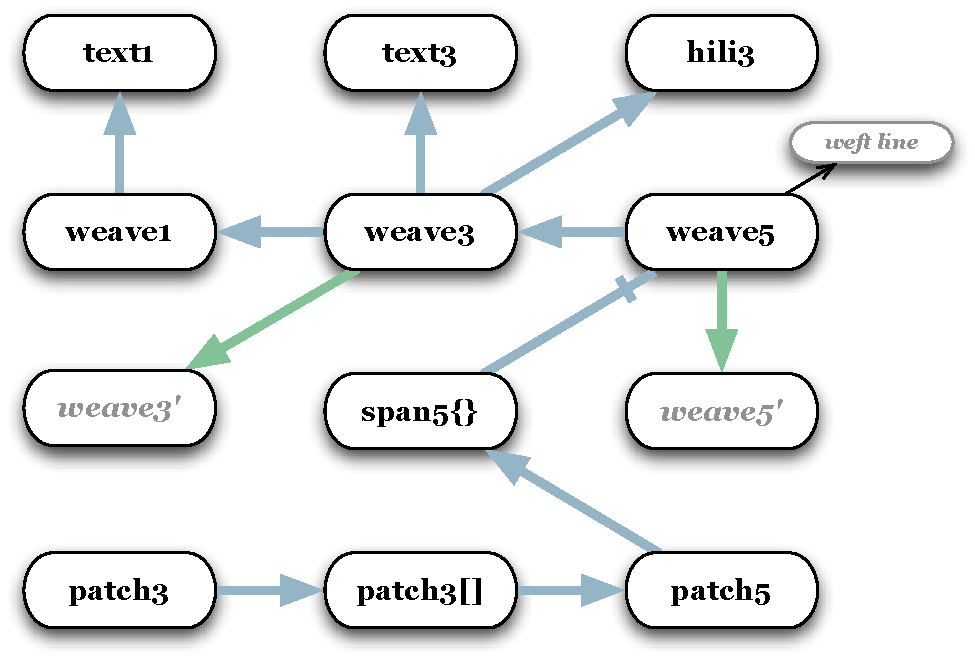
\includegraphics[width=0.48\textwidth]{formats.pdf}
\caption{Data transformations.}
\end{figure}

\paragraph{Position regex} is a technique for finding an atom in a weave without manual iteration. For a {\tt weave3}, a single-atom position regex looks like \verb+/(...)*?(.(\u0001\u0010))/+, i.e. look for atom 0x10 of the feed 1. To prevent the regex from looking for matches across atom boundaries, a weave must be terminated with a guaranteed match. In is possible to look for several atoms in one go by combining their positions with ``or'': \verb+/(...)*?(.(\u0001\u0010|\u0002\u0020))/+. As the regex employs only local backtrackings, its complexity is linear.

\paragraph{Composing a weave}

While all other operations are implemented more or less trivially once you have a weave, weave composition/patching is the most complicated algorithm. First of all, a weave is always \emph{patched}, the corner case of composition is no different as an empty weave contains the aum symbol and thus could be patched to its latest state.

Patching is done with \emph{spans}. Span is a chunk of a feed where every next atom is caused by the previous one, with an obvious exception of the very first atom. Thus, assuming that the cause of the span's first atom is already in the weave, we might insert the span as it is.
Spans allow to process atoms in bulk, avoiding symbol-by-symbol iteration, which might be expensive in a scripted language. A span corresponds to a user's period of uninterrupted typing.

Thus, the  simplest algorithm to patch a weave is:
\begin{verbatim}
1. break up patches into a queue of spans
   (abide the awareness order)
2. dequeue spans which are caused by atoms
   already in the weave
3. compose a position-regex to find all
   such causing atoms
4. run the regex over the weave to find the
   causing atoms and to insert the patches
5. while the queue is not empty, goto 2
\end{verbatim}
In the worst case, this algorithm leads to $O(N^{2})$ operations, for a weave of $N$ atoms.
A slightly more complicated algorithm employs stacks to preassemble spans before inserting them into the weave resulting in $O(N\log N)$ complexity (see Appendix~A).

The definite pain point of the algorithm is deletions/undeletions of long text ranges. As symbols have to be interleaved with backspaces, every backspace is a separate span and thus has to be separately processed. While the operation of mass deletion cannot be sustained for long, repeated delete-undelete cycles are quite likely. Some model optimizations are definitely possible to resolve the issue, but they may compromise the simplicity of the model. Thus, the preferred route is to implement purely technical optimizations. On one hand, in a Web setting a {\tt weave5} might be persistently stored on the server and handed to clients in its ready form. Thus, both the client and the server have only to patch the weave to reflect the current changes; they never reassemble it from scratch. On the other hand, there is no reason to restrict server-side calculations to scripted languages and regular expressions; native implementations might be used as well.


\paragraph{Applying waterlines}
Sometimes it is necessary to restore a historical version of a weave. To do so we have to remove any atoms introduced afterwards. It is done by a single replacement:
\verb+s/(.(?:\u0001[-\u0100]|\u0002[-\u0200]))|.../$1/g+

\paragraph{Weave to text}

A weave is converted to plain text once all deleted atoms are removed, all fictive symbols are removed and all metadata is removed. For a {\tt weave3}: \verb!s/...(\u0008..)+|(...)/$2/g!, then \verb+s/\u0000..|(...)/$1/g+ and finally \verb+s/(.)../$1/g+

\paragraph{Highlighting of changes} in a text employs already mentioned techniques. First, a weft line is applied to clear anything introduced after the later version, then any atom deleted before the former version is also removed. Then, insertion/deletion marks are set to the remaining atoms. {\tt hilight3} then might be transformed to highlighted HTML using another sequence of regular expressions.

\paragraph{Weft line closure} is an out-of-the-loop algorithm that calculates transitive closure of a weft line. For example, given that we are aware of some feed till its certain offset, what other feeds and their offsets are we aware of, recursively? Each iteration filters a weave according to the weft line, then separates all the mentions of other (causing) atoms and produces the next version of the weft line. Once the previous and the next versions match, we're done. ***On adversarial data, this might take $O(N^{2})$ time.

\paragraph{Detecting changes} is made trivial by the fact the program is permanently attached to the edited buffer. In such a case, every single action of the user might be tracked and transformed into atom deletions and insertions. Some heuristics help to deal with less trivial cases, such as bracing a range of text with tags or text undeletion.

\paragraph{Light weave} is a version of a weave lacking any atoms that were deleted ``long ago''. It is produced from the full weave using the already discussed weft regexes. Basically, it is a performance optimization which is related to the long-discussed ``tombstone problem''~\cite{ot}. Namely, that long-dead parts of a text must not incur performance penalty. On the server side, the tombstone problem is probably a misnomer. It is known that Google tends to save not only the current, but also all the historical versions of pages~\cite{google-history}. While it might sound expensive, consider that the Web grows exponentially. That leads to the simple conclusion that the need to keep the history adds just some constant factor to the amount of consumed storage, due to $\int e^{cx}dx = \frac{1}{c} e^{cx}$. In the case the Web grows less than exponentially, the impact of history-keeping is even less, as data storage definitely progresses exponentially~\cite{hdd}. Thus, there are no reason to purge ``tombstones'' permanently. At the same time, it makes sense to clear them before sending a weave to a user, assuming that the user is not interested in the entire history.

\section {Typical workflows}

As a typical workflow, let's consider a Web server hosting persistent version repository and a browser client accessing that repository and introducing changes. It is optionally possible to consider several federated Web servers sending each other changes in real-time or on request. Comet HTTP~\cite{comet} is supposed to be the protocol of choice both for client-server and server-to-server communications.

The server keeps a preassembled {\tt weave5} for every verse as well as {\tt feed5} for every author's contributions to the verse. Weaves are delivered to every new client as normal HTTP GET responses. Once a client has a weave, it makes a long outstanding Comet HTTP request for any new updates. That request specifies the client's current version using its weft line string. All user-contributed changes are converted to atoms on the client side and then sent to the server as a {\tt feed3} tail ({\tt patch3}) within a reqular HTTP POST. Once new modifications arrive at the server, they are appended to the appropriate feed and sent out as a response to outstanding Comet HTTP requests. Thus, all the other clients apply the patch to their weaves.

The server-to-server federation is not any different from the server-to-client case. It is sufficient for servers to maintain outstanding update requests or poll each other periodically. This way, changes might propagate in a gossip fashion.

The described workflow is based on the version of software presented in~\cite{broth-csr}.

\section{Evaluation}

Check: the French statement on the mass of deleted text

\section{Conclusions and implications}

First, once two key problems of version conrtol (diff and merge) are bruteforced, the rest of version control workflow is streamlined up to the degree of being implementable using mostly regular expressions. Thus, a \emph{simple} lightweight version control system might be routinely hosted within a web page to work instantly, in real time.

Second, the presented causal tree model also causes some implications for distributed wikis. It was a long-discussed~\cite{dht-wiki,piki} topic whether it is possible to host e.g. Wikipedia in a decentralized manner to spread the costs and to increase reliability. The CT model gives a different outlook on tradeoffs of (technically) decentralizing wikis. The classical paradigm is one writable ``master copy'' and lots of read-only ``cached copies''~\cite{steen-wiki} which have to be knocked out once they become ``stale''. Another popular approach is decentralizing load using distributed hash tables (DHT~\cite{dht-wiki}). The CT model enables a totally different paradigm based on massive replication: ``if you saw it, you have it''. No entry is precisely stale; instead, every feed might be saved for future use, and only has to be incrementally updated in some future. Updates may spread from their \emph{sources} in contagious manner, in a sense~\cite{contagious}, while no ``center'' or ``master copy'' is necessary.


Third, consider the possibility of not only technically, but also socially distributed/parallell wikis. Namely, the ability to federate wikis to propagate and filter changes among several ongoing ``editions'' of the same project. For example, we might have separate ``deletionist'' Wikipedia and ``inclusionist'' Wikipedia~\cite{delinc} and no contribution will be locked to a particular edition, as patch exchange is always possible. It is nice to imagine a world of many competing ``pedias'' nevertheless exchanging ``beneficial'' content ``mutations''. As we see from the massively distributed open source projects, many bottlenecks of software development are resolved~\cite{git} by the use of decentralized version control which allows to parallelize development, build elaborate workflows and, last but not least, to blame a particular developer for a particular contribution. As of today, those innovations were left mostly unnoticed by the wiki world.

\section{Acknowledgements}

Mikhail Volkov, Peter E

\end{document}
